
%%%%%%%%%%%%%%%%%%%%%%%%%%%%%%%%%%%%%%%%%%%%%%%%%%%%%%%%%%%%%%%%%%%%%%%%%%%%%%%%
%% ************************************************************************** %%
%% *                                Settings                                * %%
%% ************************************************************************** %%
%%%%%%%%%%%%%%%%%%%%%%%%%%%%%%%%%%%%%%%%%%%%%%%%%%%%%%%%%%%%%%%%%%%%%%%%%%%%%%%%
\documentclass{tron}

\loadglsentries{gls}
\glsaddall
\addbibresource{reference}
\usepackage{xcolor}  % Coloured text etc.
% fancy note style
% STYLE NOTES : v2.0
% additional fancy boxes
\usepackage[framemethod=TikZ]{mdframed}
%\usepackage{amsthm}

% gray color indicates [OPTIONAL READING]

%%%%%%%%%%%%%%%%%%%%%%%%%%%%%%
%Note
\newenvironment{note}[3][]{%
	\ifstrempty{#1}%
	{\mdfsetup{%
	frametitle={%
	\tikz[baseline=(current bounding box.east),outer sep=0pt]
	\node[anchor=east,rectangle,fill=#2]
	{\strut Note};}}
	}%
	{\mdfsetup{%
	frametitle={%
	\tikz[baseline=(current bounding box.east),outer sep=0pt]
	\node[anchor=east,rectangle,fill=#2]
	{\strut #1};}}%
	}%
	\mdfsetup{innertopmargin=0pt,skipabove=5pt,linecolor=#2,%
		linewidth=2pt,topline=true,%
		frametitleaboveskip=\dimexpr-\ht\strutbox\relax,
		backgroundcolor={white!90!#2}}
	\begin{mdframed}[]\relax%
	\label{#3}}{\end{mdframed}
}
\Crefname{note}{Note}{notes}

\newcommand{\createnoteenv}[6]{
	\refstepcounter{#6}%
	\ifstrempty{#1}%
	{\mdfsetup{%
	frametitle={%
	\tikz[baseline=(current bounding box.east),outer sep=0pt]
	\node[anchor=east,rectangle,fill=#3]
	{\strut #4~#5};}}
	}%
	{
		\mdfsetup{%
			frametitle={%
				\tikz[baseline=(current bounding box.east),outer sep=0pt]
				\node[anchor=east,rectangle,fill=#3]
				{\strut #4~#5:~#1};
			}
		}%
	}%
	\mdfsetup{innertopmargin=0pt,skipabove=5pt,linecolor=#3,%
	linewidth=2pt,topline=true,%
	frametitleaboveskip=\dimexpr-\ht\strutbox\relax,
	backgroundcolor={white!90!#3}}
	\begin{mdframed}[]\relax%
	\label{#2}
}

%%%%%%%%%%%%%%%%%%%%%%%%%%%%%%
%Definition
\newcounter{definition}[section] \setcounter{definition}{0}
\renewcommand{\thedefinition}{\arabic{section}.\arabic{definition}}
\newenvironment{definition}[2][]{%
	\createnoteenv{#1}{#2}{blue!40}{Definition}{\thedefinition}{definition}%
}{\end{mdframed}}
\newenvironment{definition*}[2][]{%
	\createnoteenv{#1}{#2}{gray!40}{Definition}{\thedefinition}{definition}%
}{\end{mdframed}}
\Crefname{definition}{Definition}{definitions}


%%%%%%%%%%%%%%%%%%%%%%%%%%%%%%
%theoremrem
\newcounter{theorem}[section] \setcounter{theorem}{0}
\renewcommand{\thetheorem}{\arabic{section}.\arabic{theorem}}
\newenvironment{theorem}[2][]{%
	\createnoteenv{#1}{#2}{cyan!40}{Theorem}{\thetheorem}{theorem}%
}{\end{mdframed}}
\newenvironment{theorem*}[2][]{%
	\createnoteenv{#1}{#2}{gray!40}{Theorem}{\thetheorem}{theorem}%
}{\end{mdframed}}
\Crefname{theorem}{Theorem}{theorems}

%%%%%%%%%%%%%%%%%%%%%%%%%%%%%%
%Proof
\newcounter{proof}[section]\setcounter{proof}{0}
\renewcommand{\theproof}{\arabic{section}.\arabic{proof}}
\newenvironment{proof}[2][]{%
	\createnoteenv{#1}{#2}{red!20}{Proof}{\theproof}{proof}%
}{\end{mdframed}}
\newenvironment{proof*}[2][]{%
	\createnoteenv{#1}{#2}{gray!40}{Proof}{\theproof}{proof}%
}{\end{mdframed}}
\Crefname{proof}{Proof}{proofs}


%%%%%%%%%%%%%%%%%%%%%%%%%%%%%%
%Alert
\newcounter{alert}[section]\setcounter{alert}{0}
\renewcommand{\thealert}{\arabic{section}.\arabic{alert}}
\newenvironment{alert}[2][]{%
	\createnoteenv{#1}{#2}{red!80}{Alert}{\thealert}{alert}%
}{\end{mdframed}}
\newenvironment{alert*}[2][]{%
	\createnoteenv{#1}{#2}{gray!40}{Alert}{\thealert}{alert}%
}{\end{mdframed}}
\Crefname{alert}{Alert}{alerts}

%%%%%%%%%%%%%%%%%%%%%%%%%%%%%%
%Answer
\newcounter{answer}[section]\setcounter{answer}{0}
\renewcommand{\theanswer}{\arabic{section}.\arabic{answer}}
\newenvironment{answer}[2][]{%
	\createnoteenv{#1}{#2}{orange!60}{Answer}{\theanswer}{answer}%
}{\end{mdframed}}
\newenvironment{answer*}[2][]{%
	\createnoteenv{#1}{#2}{gray!40}{Answer}{\theanswer}{answer}%
}{\end{mdframed}}
\Crefname{answer}{Answer}{answers}

%%%%%%%%%%%%%%%%%%%%%%%%%%%%%%
%Remark
\newcounter{remark}[section]\setcounter{remark}{0}
\renewcommand{\theremark}{\arabic{section}.\arabic{remark}}
\newenvironment{remark}[2][]{%
	\createnoteenv{#1}{#2}{orange!40}{Remark}{\theremark}{remark}%
}{\end{mdframed}}
\newenvironment{remark*}[2][]{%
	\createnoteenv{#1}{#2}{gray!40}{Remark}{\theremark}{remark}%
}{\end{mdframed}}
\Crefname{remark}{Remark}{remarks}


%%%%%%%%%%%%%%%%%%%%%%%%%%%%%%%
%%Example
%\newcounter{example}[section]\setcounter{example}{0}
%\renewcommand{\theexample}{\arabic{section}.\arabic{example}}
%\newenvironment{example}[2][]{%
%	\createnoteenv{#1}{#2}{blue!40!cyan!20}{Example}{\theexample}{example}%
%}{\end{mdframed}}
%\newenvironment{example*}[2][]{%
%	\createnoteenv{#1}{#2}{gray!40}{Example}{\theexample}{example}%
%}{\end{mdframed}}

%%%%%%%%%%%%%%%%%%%%%%%%%%%%%%
%Algorithm
\newcounter{algo}[section]\setcounter{algo}{0}
\renewcommand{\thealgo}{\arabic{algo}.\arabic{algo}}
\newenvironment{algo}[2][]{%
	\createnoteenv{#1}{#2}{yellow!90!brown!60}{Algorithm}{\thealgo}{algo}%
}{\end{mdframed}}
\newenvironment{algo*}[2][]{%
	\createnoteenv{#1}{#2}{gray!40}{Algorithm}{\thealgo}{algo}%
}{\end{mdframed}}
\Crefname{algo}{Algorithm}{algos}

%%%%%%%%%%%%%%%%%%%%%%%%%%%%%%
% CS480 - Exercise
%\setlength{\parskip}{1cm}
%\setlength{\parindent}{1cm}

%\tikzstyle{titregris} =
%[draw=gray,fill=white, shading = exersicetitle, %
%text=gray, rectangle, rounded corners, right,minimum height=.3cm]
%\pgfdeclarehorizontalshading{exersicebackground}{100bp}
%{color(0bp)=(green!40); color(100bp)=(black!5)}
%\pgfdeclarehorizontalshading{exersicetitle}{100bp}
%{color(0bp)=(red!40);color(100bp)=(black!5)}
%\newcounter{exercise}
%\renewcommand*\theexercise{exercice \textbf{Exercice}~n\arabic{exercise}}
%\makeatletter
%\def\mdf@@exercisepoints{}%new mdframed key:
%\define@key{mdf}{exercisepoints}{%
%\def\mdf@@exercisepoints{#1}
%}
%
%\mdfdefinestyle{theoremstyle}{%
%outerlinewidth=0.01em,linecolor=black,middlelinewidth=0.5pt,%
%frametitlerule=true,roundcorner=2pt,%
%apptotikzsetting={\tikzset{mfframetitlebackground/.append style={%
%shade,left color=white, right color=blue!20}}},
%frametitlerulecolor=black,innertopmargin=1\baselineskip,%green!60,
%innerbottommargin=0.5\baselineskip,
%frametitlerulewidth=0.1pt,
%innertopmargin=0.7\topskip,skipabove={\dimexpr0.2\baselineskip+0.1\topskip\relax},
%frametitleaboveskip=1pt,
%frametitlebelowskip=1pt
%}
%\mdtheorem[style=theoremstyle]{exercise}{\textbf{Exercise}}

\newcounter{exercise}[section]\setcounter{exercise}{0}
\renewcommand{\theexercise}{\arabic{exercise}}
\newenvironment{exercise}[2][]{%
	\createnoteenv{#1}{#2}{gray!40}{Exercise}{\theexercise}{exercise}%
}{\end{mdframed}}
\newenvironment{exercise*}[2][]{%
	\createnoteenv{#1}{#2}{gray!40}{Exercise}{\theexercise}{exercise}%
}{\end{mdframed}}

\Crefname{exercise}{Exercise}{exercises}


%%%%%%%%%%%%%%%%%%%%%%%%%%%%%%
%Examples
% {

%     \section{Theorem and lemma examples with title}
%     \begin{theorem}[Pythagoras' theorem]{theorem:pythagoras}
%     In a right triangle, the square of the hypotenuse is equal to the sum of the squares of the catheti.
%     \[a^2+b^2=c^2\]
%     \end{theorem}
%     In mathematics, the Pythagorean theorem, also known as Pythagoras' theorem (see theorem \ref{theorem:pythagoras}), is a relation in Euclidean geometry among the three sides of a right triangle.
%     
%     \begin{definition}[B\'ezout's identity]{def:bezout}
%     Let $a$ and $b$ be nonzero integers and let $d$ be their greatest common divisor. Then there exist integers $x$ and $y$ such that:
%     \[ax+by=d\]
%     \end{definition}
%     This is a reference to Bezout's lemma \ref{def:bezout}
%     
%     
%     \section{Theorem and proof examples without title}
%     
%     \begin{theorem}[]{theorem:theorem1}
%     There exist two irrational numbers $x$, $y$ such that $x^y$ is rational.
%     \end{theorem}
%     
%     \begin{proof}[]{proof:proof1}
%     If $x=y=\sqrt{2}$ is an example, then we are done; otherwise $\sqrt{2}^{\sqrt{2}}$ is irrational, in which case taking $x=\sqrt{2}^{\sqrt{2}}$ and $y=\sqrt{2}$ gives us:
%     \[\bigg(\sqrt{2}^{\sqrt{2}}\bigg)^{\sqrt{2}}=\sqrt{2}^{\sqrt{2}\sqrt{2}}=\sqrt{2}^{2}=2.\]
%     \end{proof}
%
%     \begin{alert}[]{alert:alert1}
%     If $x=y=\sqrt{2}$ is an example, then we are done; otherwise $\sqrt{2}^{\sqrt{2}}$ is irrational, in which case taking $x=\sqrt{2}^{\sqrt{2}}$ and $y=\sqrt{2}$ gives us:
%     \[\bigg(\sqrt{2}^{\sqrt{2}}\bigg)^{\sqrt{2}}=\sqrt{2}^{\sqrt{2}\sqrt{2}}=\sqrt{2}^{2}=2.\]
%     \end{alert}
%     
%     \begin{remark}[]{alert:alert1}
%     If $x=y=\sqrt{2}$ is an example, then we are done; otherwise $\sqrt{2}^{\sqrt{2}}$ is irrational, in which case taking $x=\sqrt{2}^{\sqrt{2}}$ and $y=\sqrt{2}$ gives us:
%     \[\bigg(\sqrt{2}^{\sqrt{2}}\bigg)^{\sqrt{2}}=\sqrt{2}^{\sqrt{2}\sqrt{2}}=\sqrt{2}^{2}=2.\]
%     \end{remark}
%     
%     
%          \begin{exercise}[]{alert:alert1}
%     If $x=y=\sqrt{2}$ is an example, then we are done; otherwise $\sqrt{2}^{\sqrt{2}}$ is irrational, in which case taking $x=\sqrt{2}^{\sqrt{2}}$ and $y=\sqrt{2}$ gives us:
%     \[\bigg(\sqrt{2}^{\sqrt{2}}\bigg)^{\sqrt{2}}=\sqrt{2}^{\sqrt{2}\sqrt{2}}=\sqrt{2}^{2}=2.\]
%     \end{exercise}
%     
%     \begin{algo}[]{algorithm:alert1}
%     If $x=y=\sqrt{2}$ is an example, then we are done; otherwise $\sqrt{2}^{\sqrt{2}}$ is irrational, in which case taking $x=\sqrt{2}^{\sqrt{2}}$ and $y=\sqrt{2}$ gives us:
%     \[\bigg(\sqrt{2}^{\sqrt{2}}\bigg)^{\sqrt{2}}=\sqrt{2}^{\sqrt{2}\sqrt{2}}=\sqrt{2}^{2}=2.\]
%     \end{algo}
%     
%     \begin{note}[Goal]{pink}{note:goal}
%     If $x=y=\sqrt{2}$ is an example, then we are done; otherwise $\sqrt{2}^{\sqrt{2}}$ is irrational, in which case taking $x=\sqrt{2}^{\sqrt{2}}$ and $y=\sqrt{2}$ gives us:
%     \[\bigg(\sqrt{2}^{\sqrt{2}}\bigg)^{\sqrt{2}}=\sqrt{2}^{\sqrt{2}\sqrt{2}}=\sqrt{2}^{2}=2.\]
%     \end{note}

% }
%\usepackage{lipsum}                     % Dummytext
\usepackage{xargs}                      % Use more than one optional parameter in a new commands
\usepackage[colorinlistoftodos,prependcaption,textsize=normalsize]{todonotes}
%
\newcommandx{\unsure}[2][1=]{\todo[linecolor=red,backgroundcolor=red!25,bordercolor=red,#1]{#2}}
\newcommandx{\change}[2][1=]{\todo[linecolor=blue,backgroundcolor=blue!25,bordercolor=blue,#1]{#2}}
\newcommandx{\info}[2][1=]{\todo[linecolor=OliveGreen,backgroundcolor=OliveGreen!25,bordercolor=OliveGreen,#1]{#2}}
\newcommandx{\improvement}[2][1=]{\todo[linecolor=Plum,backgroundcolor=Plum!25,bordercolor=Plum,#1]{#2}}
\newcommandx{\thiswillnotshow}[2][1=]{\todo[disable,#1]{#2}}
%
\preto\printlistoftodos{
    \listoftodos[Todo List]
}

% EXAMPLES:
    % \todo[inline]{The original todo note withouth changed colours.\newline Here's another line.}
    % \lipsum[11]\unsure{Is this correct?}\unsure{I'm unsure about also!}
    % \lipsum[11]\change{Change this!}
    % \lipsum[11]\info{This can help me in chapter seven!}
    % \lipsum[11]\improvement{This really needs to be improved!\newline\newline What was I thinking?!}
    % \lipsum[11]
    % \thiswillnotshow{This is hidden since option `disable' is chosen!}
    % \improvement[inline]{The following section needs to be rewritten!}
    % \lipsum[11]
    % \newpage
    % \listoftodos[Notes]
%%%  Equation Condition
\newenvironment{eqconditions}
  {\par\vspace{\abovedisplayskip}\noindent\begin{tabular}{>{$}l<{$} @{${}={}$} l}}
  {\end{tabular}\par\vspace{\belowdisplayskip}}
\newenvironment{eqconditions*}
  {\noindent\begin{tabular}{>{$}l<{$} @{${}={}$} l}}
  {\end{tabular}}
%%% introduce 4th depth with \paragraph command
\usepackage{titlesec}
\setcounter{secnumdepth}{4}
\titleformat{\paragraph}
{\normalfont\normalsize\bfseries}{\theparagraph}{1em}{}
\titlespacing*{\paragraph}
{0pt}{3.25ex plus 1ex minus .2ex}{1.5ex plus .2ex}

%%% enumeration reference
% constraint
\newlist{constraint-list}{enumerate}{1}
\setlist[constraint-list,1]{leftmargin=*, label= \Roman*}
\creflabelformat{Constraint}{#2#1#3}
\crefname{constraint-listi}{Constraint}{position}
% criteria
\newlist{criteria-list}{enumerate}{1}
\setlist[criteria-list,1]{leftmargin=*, label= \Roman*}
\creflabelformat{Criterion}{#2#1#3}
\crefname{criteria-listi}{Criterion}{position}
% property
\newlist{property-list}{enumerate}{1}
\setlist[property-list,1]{leftmargin=*, label= \Roman*}
\creflabelformat{Property}{#2#1#3}
\crefname{property-listi}{Property}{position}
% assumption
\newlist{assumption-list}{enumerate}{1}
\setlist[assumption-list,1]{leftmargin=*, label= \Roman*}
\creflabelformat{Assumption}{#2#1#3}
\crefname{assumption-listi}{Assumption}{position}

% custom math command
\newcommand{\unit}[1]{\left[\si{#1}\right]}

% additional math packages
\usepackage{physics}
\usepackage{cancel}

% TODO Flags
\newcommand\TODO[1]{{\textcolor{red}{\textbf{#1}}}}
\newcommand\COMMENT[1]{\hl{#1}}

% Custom Format
% \usepackage{float}
% \usepackage[table]{xcolor}
% \usepackage{soul}
\usepackage{multirow}
\usepackage{caption} 
\captionsetup[table]{skip=3pt}
\captionsetup[figure]{skip=0pt}
\titlespacing*{\section}
{0pt}{10pt}{3pt}
\titlespacing*{\subsection}
{0pt}{8pt}{3pt}
\titlespacing*{\subsubsection}
{0pt}{8pt}{3pt}
%hide the highlight box
\hypersetup{
    colorlinks,
    linkcolor={black!50!black},
    citecolor={black!50!blue},
    urlcolor={black!80!black}
}%hide the highlight box

% table formatting
% \setlength{\arrayrulewidth}{1mm}
% \setlength{\tabcolsep}{18pt}
% \renewcommand{\arraystretch}{2.5}
\usepackage{array}
\newcolumntype{C}[1]{>{\centering\let\newline\\\arraybackslash\hspace{0pt}}m{#1}}

% custom math symbol
%% CS 480 %%
\newcommand{\bm}[1]{\mathbf{#1}}
%%%%%%%%%%%%
\newcommand{\RR}{\mathds{R}}
\newcommand{\Id}{\mathbb{I}}
\newcommand{\NN}{\mathds{N}}
\newcommand{\sign}{\mathop{\mathrm{sign}}}
\newcommand{\diag}{\mathop{\mathrm{diag}}}
\newcommand{\argmin}{\mathop{\mathrm{argmin}}}
\newcommand{\zero}{\mathbf{0}}
\newcommand{\one}{\mathbf{1}}
\newcommand{\av}{\mathbf{a}}
\newcommand{\bv}{\mathbf{b}}
\newcommand{\sv}{\mathbf{s}}
\newcommand{\Xv}{\mathbf{X}}
\newcommand{\Yv}{\mathbf{Y}}
\newcommand{\wv}{\mathbf{w}}
\newcommand{\xv}{\mathbf{x}}
\newcommand{\yv}{\mathbf{y}}
\newcommand{\zv}{\mathbf{z}}
\newcommand{\uv}{\mathbf{u}}
\newcommand{\rv}{\mathbf{r}}
\newcommand{\inner}[2]{\langle #1, #2 \rangle}
\newcommand{\red}[1]{{\color{red}#1}}
\newcommand{\blue}[1]{{\color{blue}#1}}
\newcommand{\magenta}[1]{{\color{magenta}#1}}


\newcommand{\ea}{{et al.}\xspace}
\newcommand{\eg}{{e.g.}\xspace}
\newcommand{\ie}{{i.e.}\xspace}
\newcommand{\iid}{{i.i.d.}\xspace}
\newcommand{\cf}{{cf.}\xspace}
\newcommand{\wrt}{{w.r.t.}\xspace}
\newcommand{\aka}{{a.k.a.}\xspace}
\newcommand{\etc}{{etc.}\xspace}
\newcommand{\sgm}{\mathsf{sgm}}
\newcommand{\Dc}{\mathcal{D}}
\newcommand{\ans}[1]{{\textcolor{orange}{\textsf{Ans}: #1}}}



% extra mod
\newcommand{\mref}[1]{\underline{\textbf{\hypersetup{linkcolor=orange}\Cref{#1}\hypersetup{linkcolor=blue}}}}

%%%%%%%%%%%%%%%%%%%%%%%%%%%%%%%%%%%%%%%%%%%%%%%%%%%%%%%%%%%%%%%%%%%%%%%%%%%%%%%%
% Make sure the following block contains the correct information               %
%%%%%%%%%%%%%%%%%%%%%%%%%%%%%%%%%%%%%%%%%%%%%%%%%%%%%%%%%%%%%%%%%%%%%%%%%%%%%%%%
\reporttitle{CS 480 - Homework 1}
% \selfstudy % comment this line if this is not a self study report 
% \employername{Employer Name}
% \employerstreetaddress{Employer Address}
% \employerlocation{City, Provice, Country}
\university{University of Waterloo}
\faculty{Cheriton School of Computer Science}%Faculty of Engineering
\department{}%Department of Systems Design Engineering
\groupnumber{1}
\authornameA{Jianxiang (Jack) Xu}
\studentnumberA{20658861}
\reportdate{\today}
%\confidential{1} % comment this line if this is not a confidential report
%\authorstreetaddress{##}
%\authorlocation{##}
%\authorpostalcode{##}
\useheader % comment this line if no need for header
%%%%%%%%%%%%%%%%%%%%%%%%%%%%%%%%%%%%%%%%%%%%%%%%%%%%%%%%%%%%%%%%%%%%%%%%%%%%%%%%
% end of information block...                                                  %
%%%%%%%%%%%%%%%%%%%%%%%%%%%%%%%%%%%%%%%%%%%%%%%%%%%%%%%%%%%%%%%%%%%%%%%%%%%%%%%%

\begin{document}
%%%%%%%%%%%%%%%%%%%%%%%%%%%%%%%%%%%%%%%%%%%%%%%%%%%%%%%%%%%%%%%%%%%%%%%%%%%%%%%%
%% ************************************************************************** %%
%% *                               Title Page                               * %%
%% ************************************************************************** %%
%%%%%%%%%%%%%%%%%%%%%%%%%%%%%%%%%%%%%%%%%%%%%%%%%%%%%%%%%%%%%%%%%%%%%%%%%%%%%%%%
\maketitle
%%%%%%%%%%%%%%%%%%%%%%%%%%%%%%%%%%%%%%%%%%%%%%%%%%%%%%%%%%%%%%%%%%%%%%%%%%%%%%%%
%% ************************************************************************** %%
%% *                           Table of Contents                            * %%
%% ************************************************************************** %%
%%%%%%%%%%%%%%%%%%%%%%%%%%%%%%%%%%%%%%%%%%%%%%%%%%%%%%%%%%%%%%%%%%%%%%%%%%%%%%%%
% \tableofcontents
%%%%%%%%%%%%%%%%%%%%%%%%%%%%%%%%%%%%%%%%%%%%%%%%%%%%%%%%%%%%%%%%%%%%%%%%%%%%%%%%
%% ************************************************************************** %%
%% *                            List of Figures                             * %%
%% ************************************************************************** %%
%%%%%%%%%%%%%%%%%%%%%%%%%%%%%%%%%%%%%%%%%%%%%%%%%%%%%%%%%%%%%%%%%%%%%%%%%%%%%%%%
% \listoffigures
%%%%%%%%%%%%%%%%%%%%%%%%%%%%%%%%%%%%%%%%%%%%%%%%%%%%%%%%%%%%%%%%%%%%%%%%%%%%%%%%
%% ************************************************************************** %%
%% *                             List of Tables                             * %%
%% ************************************************************************** %%
%%%%%%%%%%%%%%%%%%%%%%%%%%%%%%%%%%%%%%%%%%%%%%%%%%%%%%%%%%%%%%%%%%%%%%%%%%%%%%%%
% \listoftables
%%%%%%%%%%%%%%%%%%%%%%%%%%%%%%%%%%%%%%%%%%%%%%%%%%%%%%%%%%%%%%%%%%%%%%%%%%%%%%%%
%% ************************************************************************** %%
%% *                              MAIN BODY                                 * %%
%% ************************************************************************** %%
%%%%%%%%%%%%%%%%%%%%%%%%%%%%%%%%%%%%%%%%%%%%%%%%%%%%%%%%%%%%%%
\clearpage
\pagenumbering{arabic}
\setcounter{page}{1}
\setlength{\parskip}{5pt}
\newpage

%%%%%%%%%%%%%%%%%%%%%%%%%%%%%%%%%%%
%%%%% Intro.  %%%%%%
%%%%%%%%%%%%%%%%%%%%%%%%%%%%%%%%%%%
\begin{center}
  \large{\textbf{CS480/680: Introduction to Machine Learning} \\ Homework 2\\ \red{Due: 11:59 pm, February 12, 2021}}
\end{center}


%%%%%%%%%%%%%%%%
%%%%% Ex 1 %%%%%
%%%%%%%%%%%%%%%%
\setcounter{section}{1}
\begin{exercise}[CNN Implementation (8 pts)]{}
	\blue{\textbf{Note}: Please mention your Python version (and maybe the version of all other packages).}
	
	% In this exercise you are going to run some experiments involving CNNs. You need to know \href{https://www.python.org/}{\magenta{Python}} and install the following libraries: \href{https://keras.io/}{\magenta{Keras}}, \href{https://www.tensorflow.org/install/}{\magenta{Tensorflow}}, \href{http://www.numpy.org/}{\magenta{Numpy}} and all their dependencies. You can find detailed instructions and tutorials for each of these libraries on the respective websites. 
	% [To install, try \textsf{pip install keras}. For Tensorflow, follow the installation steps on its webpage.]
	
	In this exercise you are going to run some experiments involving CNNs. You need to know \href{https://www.python.org/}{\magenta{Python}} and install the following libraries: \href{https://pytorch.org/get-started/locally/}{\magenta{Pytorch}}, \href{https://matplotlib.org/}{\magenta{matplotlib}} and all their dependencies. You can find detailed instructions and tutorials for each of these libraries on the respective websites. 
	
	For all experiments, running on CPU is sufficient. You do not need to run the code on GPUs.
	% Before start, we suggest you review what we learned about each layer in CNN, and read at least this \href{https://keras.io/getting-started/sequential-model-guide/}{\magenta{tutorial}}.
	Before start, we suggest you review what we learned about each layer in CNN, and read at least this \href{https://pytorch.org/tutorials/beginner/blitz/neural_networks_tutorial.html}{\magenta{tutorial}}.
	
	\begin{enumerate}
		\item Train a VGG11 net on the \href{https://pytorch.org/vision/0.9/datasets.html#mnist}{\magenta{MNIST}} dataset. 
		VGG11 was an earlier version of VGG16 and can be found as model A in Table 1 of this \href{https://arxiv.org/pdf/1409.1556.pdf}{\magenta{paper}}, whose Section 2.1 also gives you all the details about each layer.
		The goal is to get the loss as close to 0 loss as possible. Note that our input dimension is different from the VGG paper. You need to resize each image in MNIST from its original size $28 \times 28$ to $32 \times 32$ [make sure you understand why this is].
		
		For your convenience, we list the details of the VGG11 architecture here.
		The convolutional layers are denoted as \texttt{Conv(number of input channels, number of output channels, kernel size, stride, padding)};
		the batch normalization layers  are denoted as \texttt{BatchNorm(number of channels)};
		the max-pooling layers are denoted as \texttt{MaxPool(kernel size, stride)};
		the fully-connected layers are denoted as \texttt{FC(number of input features, number of output features)};
		the drop out layers are denoted as \texttt{Dropout(dropout ratio)}:
		\begin{verbatim}
		- Conv(001, 064, 3, 1, 1) - BatchNorm(064) - ReLU - MaxPool(2, 2)
		- Conv(064, 128, 3, 1, 1) - BatchNorm(128) - ReLU - MaxPool(2, 2)
		- Conv(128, 256, 3, 1, 1) - BatchNorm(256) - ReLU 
		- Conv(256, 256, 3, 1, 1) - BatchNorm(256) - ReLU - MaxPool(2, 2)
		- Conv(256, 512, 3, 1, 1) - BatchNorm(512) - ReLU 
		- Conv(512, 512, 3, 1, 1) - BatchNorm(512) - ReLU - MaxPool(2, 2)
		- Conv(512, 512, 3, 1, 1) - BatchNorm(512) - ReLU 
		- Conv(512, 512, 3, 1, 1) - BatchNorm(512) - ReLU - MaxPool(2, 2)
		- FC(0512, 4096) - ReLU - Dropout(0.5) 
		- FC(4096, 4096) - ReLU - Dropout(0.5) 
		- FC(4096, 10)
		\end{verbatim}
		You should use the \href{https://pytorch.org/docs/master/generated/torch.nn.CrossEntropyLoss.html}{cross-entropy loss} \verb|torch.nn.CrossEntropyLoss| at the end.
		
		[This experiment will take up to 1 hour on a CPU, so please be cautious of your time. If this running time is not bearable, you may cut the training set to 1/10, so only have $\sim$600 images per class instead of the regular $\sim$6000.]
		
		\item Once you've done the above, the next goal is to inspect the training process. Create the following plots:
		\begin{enumerate}
			\item (1 pt) test accuracy vs the number of epochs (say 3 $\sim$ 5)
			\item (1 pt) training accuracy vs the number of epochs
			\item (1 pt) test loss vs the number of epochs
			\item (1 pt) training loss vs the number of epochs
		\end{enumerate}
		[If running more than 1 epoch is computationally infeasible, simply run 1 epoch and try to record the accuracy/loss after every few minibatches.]
		
		\ans{\mref{ans:1:1}}
		
		\item Then, it is time to inspect the generalization properties of your final model. Flip and blur the \red{test set images} using any python library of your choice, and complete the following:		
		\begin{enumerate}[resume]
			\item (1 pt) test accuracy vs type of flip. Try the following two types of flipping: flip each image from left to right, and from top to bottom. Report the test accuracy after each flip. What is the effect? Please explain the effect in one sentence.
			
			You can read this \href{https://pytorch.org/vision/stable/transforms.html}{\magenta{doc}} to learn how to build a complex transformation pipeline. We suggest the following command for performing flipping: 
			\begin{verbatim}
			torchvision.transforms.RandomHorizontalFlip(p=1)
			torchvision.transforms.RandomVerticalFlip(p=1)
			\end{verbatim}
			
			\ans{}
			
			\item (1 pt) test accuracy vs Gaussian noise. Try adding standard Gaussian noise to each test image with variance 0.01, 0.1, 1 and report the test accuracies. What is the effect? Please explain the effect in one sentence.
			
			For instance, you may apply a user-defined lambda as a new transform t which adds Gaussian noise with variance say 0.01: 
			\begin{verbatim}
			t = torchvision.transforms.Lambda(lambda x : x + 0.1*torch.randn_like(x))
			\end{verbatim}
			
			\ans{}
		\end{enumerate} 
		
		\item (2 pts) Lastly, let us verify the effect of regularization. Retrain your model with data augmentation and test again as in part 3. Report the test accuracies and explain what kind of data augmentation you use in retraining.
		
		\ans{}
		
	\end{enumerate}
	
\end{exercise}
% --- ANS --- %
\begin{answer}[VGG11 Implementation]{ans:1:1}
%	Note: 
%	- https://www.programmersought.com/article/98065176727/
%	- https://blog.csdn.net/zhaoyin214/article/details/106350049


%	{	
%			\centering
%			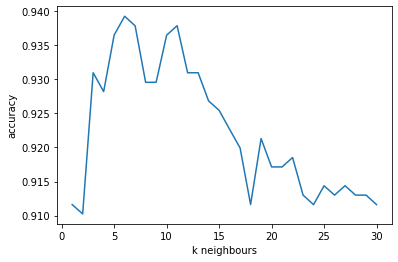
\includegraphics[height=200px]{Fig/q1}
%	      	\captionof{figure}{KNN Accuracy vs. K-size  \label{fig:q1:1:knn}}
%	}	
%	\textbf{See code in the jupyter submission.}
\end{answer}

% --- ANS --- %
\begin{answer}[TODO]{ans:1:2}
\end{answer}

% --- ANS --- %
\begin{answer}[TODO]{ans:1:3}
\end{answer}

% --- ANS --- %
\begin{answer}[TODO]{ans:1:4}
\end{answer}



%%%%%%%%%%%%%%%
%%%% Ex 2 %%%%%
%%%%%%%%%%%%%%%
\newpage
\setcounter{section}{2}
\begin{exercise}[Gaussian Mixture Model (GMM) (10 pts)]{}
	\blue{\textbf{Notation}: For a matrix $A$, $|A|$ denotes its \href{https://en.wikipedia.org/wiki/Determinant}{\magenta{determinant}}. For a \href{https://en.wikipedia.org/wiki/Diagonal_matrix}{\magenta{diagonal matrix}} $\diag(\sv)$, $|\diag(\sv)| = \prod_{i} s_i$.}
	
	\begin{algorithm}[H]
		\DontPrintSemicolon
		\KwIn{$X\in\RR^{n\times d}$, $K\in \NN$, initialization for $model$}
		\tcp{$model$ includes $\pi\in\RR^K_+$ and for each $1\leq k \leq K$, $\boldsymbol{\mu}_k \in \RR^d$ and $S_k\in\mathbb{S}^d_+$}
		\tcp{$\pi_k \geq 0$, $\sum_{k=1}^K \pi_k = 1$, $S_k$ symmetric and positive definite.}
		\tcp{random initialization suffices for full credit.}
		\tcp{alternatively, can initialize $r$ by randomly assigning each data to one of the $K$ components}
		\KwOut{$model, \ell$}
		
		\For{$iter = 1: \textsc{maxiter}$}{
			\tcp{step 2, for each $i=1,\ldots, n$}
			\For{$k=1, \ldots, K$}{
				\red{$r_{ik} \gets \pi_k |S_k|^{-1/2} \exp[-\frac{1}{2} (\xv_i - \boldsymbol{\mu}_k)^\top S_k^{-1}(\xv_i - \boldsymbol{\mu}_k)]$} \tcp*{compute responsibility}			
			}
			
			\tcp{for each $i=1,\ldots, n$}
			$r_{i.} \gets \sum_{k=1}^K r_{ik}$
			
			\tcp{for each $k=1, \ldots, K$ and $i=1,\ldots, n$}		
			$r_{ik} \gets r_{ik} / r_{i.}$ \tcp*{normalize}
			
			\tcp{compute negative log-likelihood}
			$\ell(iter) = -\sum_{i=1}^n \log(r_{i.})$
			
			\If{$iter > 1 ~\&\&~ |\ell(iter)-\ell(iter-1)| \leq \textsc{tol}*|\ell(iter)|$}{
				\textbf{break}
			}
			
			\tcp{step 1, for each $k=1, \ldots, K$}
			$r_{.k} \gets \sum_{i=1}^n r_{ik}$
			
			$\pi_k \gets r_{.k} / n$
			
			$\boldsymbol{\mu}_k = \sum_{i=1}^n r_{ik} \xv_i / r_{.k}$
			
			\red{$S_k \gets \left(\sum_{i=1}^n r_{ik} \xv_i \xv_i^\top / r_{.k}\right) - \boldsymbol{\mu}_k \boldsymbol{\mu}_k^\top$}
		}
		\caption{EM for GMM.}
		\label{alg:gmm}
	\end{algorithm}
	
	\begin{enumerate}
		\item (2 pts) Derive and implement the EM algorithm for the \blue{diagonal} Gaussian mixture model, \red{where all covariance matrices are constrained to be diagonal}. \Cref{alg:gmm} recaps all the essential steps and serves as a hint rather than a verbatim instruction. In particular, you must change the highlighted steps accordingly (with each $S_k$ being a diagonal matrix), along with formal explanations. Analyze the space and time complexity of your implementation. 
		
		[You might want to review the steps we took in class (lecture 16) to get the updates in \Cref{alg:gmm} and adapt them to the simpler case here. The solution should look like $s_j = \frac{\sum_{i=1}^n r_{ik} (x_{ij} - \mu_j)^2}{\sum_{i=1}^n r_{ik} } = \frac{\sum_{i=1}^n r_{ik} x_{ij} ^2}{\sum_{i=1}^n r_{ik} } - \mu_j^2$ for the $j$-th diagonal. Multiplying an $n\times p$ matrix with a $p\times m$ matrix costs $O(mnp)$. Do not maintain a diagonal matrix explicitly; using a vector for its diagonal suffices.]
		
		To stop the algorithm, set a maximum number of iterations (say $\textsc{maxiter} = 500$) and also monitor the change of the negative log-likelihood $\ell$: 
		\begin{align}
		\ell = -\sum_{i=1}^n \log\left[\sum_{k=1}^K \pi_k |2\pi S_k|^{-1/2} \exp[ -\tfrac{1}{2}(\xv_i -\boldsymbol{\mu}_k)^\top S_k^{-1} (\xv_i - \boldsymbol{\mu}_k ) ]\right],
		\end{align}
		where $\xv_i$ is the $i$-th column of $X^\top$.
		\blue{As a debug tool, note that $\ell$ should decrease from step to step}, and we can stop the algorithm if the decrease is smaller than a predefined threshold, say $\textsc{tol} = 10^{-5}$.
		
		\ans{}
			
		\item (2 pts) Redo Ex 2.1 with the \blue{spherical} Gaussian mixture model, where each covariance matrix $S_k = s_k I$ is a multiple of the identity matrix $I$. Derive the update for $s_k$ and implement the resulting EM algorithm. Analyze the space and time complexity of your implementation.
		
		\ans{}
				
		\item (2 pts) Redo Ex 2.1 where we fit $d$ GMMs (each with $K$ components) to each feature $X_{:,j}$, separately. Implement the resulting EM algorithm. Analyze the space and time complexity of your implementation.
		
		\ans{}
		
		\item (4 pts) Next, we apply (the adapted) \Cref{alg:gmm} in Ex 2.1 to the \href{https://pytorch.org/vision/0.9/datasets.html#mnist}{\magenta{MNIST}} dataset. For each of the 10 classes (digits), we can use its (only its) training images to estimate its (class-conditional) distribution by fitting a GMM (with say $K=5$, roughly corresponding to 5 styles of writing this digit). This gives us the density estimate $p(\xv | y)$ where $\xv$ is an image (of some digit) and $y$ is the class (digit). We can now classify the test set using the Bayes classifier:
		\begin{align}
		\hat y(\xv) = \arg\max_{c = 0, \ldots, 9} ~~ \underbrace{\mathrm{Pr}(Y = c) \cdot p(X = \xv | Y = c)}_{\propto ~\mathrm{Pr}(Y=c | X=\xv)},
		\end{align}
		where the probabilities $\mathrm{Pr}(Y = c)$ can be estimated using the training set, \eg, the proportion of the $c$-th class in the training set, and the \red{density} $p(X = \xv | Y = c)$ is estimated using GMM for each class $c$ separately. Report your error rate on the test set as a function of $K$ (if time is a concern, using $K=5$ will receive  full credit). 
		
		[Optional: Reduce dimension by \href{https://en.wikipedia.org/wiki/Principal_component_analysis}{\magenta{PCA}} may boost accuracy quite a bit. Your running time should be on the order of minutes (for one $K$), if you do not introduce extra for-loops in \Cref{alg:gmm}.]
		
		[In case you are wondering, our classification procedure above belongs to the so-called plug-in estimators (plug the estimated densities to the known optimal Bayes classifier). However, note that estimating the density $p(X=\xv | Y = c)$ is actually harder than classification. Solving a problem (\eg classification) through some intermediate harder problem (\eg density estimation) is almost always a bad idea.]
		
		\ans{}
		

	\end{enumerate}	
\end{exercise}
% --- ANS --- %
\begin{answer}[TODO]{ans:2:1}
%	{	
%			\centering
%			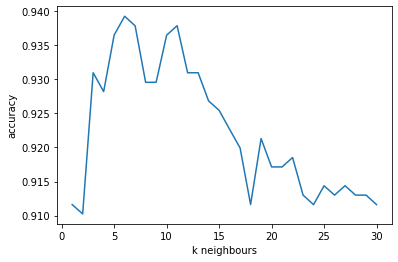
\includegraphics[height=200px]{Fig/q1}
%	      	\captionof{figure}{KNN Accuracy vs. K-size  \label{fig:q1:1:knn}}
%	}	
%	\textbf{See code in the jupyter submission.}
\end{answer}

% --- ANS --- %
\begin{answer}[TODO]{ans:2:2}
\end{answer}

% --- ANS --- %
\begin{answer}[TODO]{ans:2:3}
\end{answer}

% --- ANS --- %
\begin{answer}[TODO]{ans:2:4}
\end{answer}

%%%%%%%%%%%%%%%%%%%%%%%%%%%%%%%%%%%%%%%%%%%%%%%%%%%%%%%%%%%%%%%%%%%%%%%%%%%%%%%%
%% ************************************************************************** %%
%% *                      TODO [Remove For Final Copy!]                     * %%
%% ************************************************************************** %%
%%%%%%%%%%%%%%%%%%%%%%%%%%%%%%%%%%%%%%%%%%%%%%%%%%%%%%%%%%%%%%%%%%%%%%%%%%%%%%%%
%\printlistoftodos

%%%%%%%%%%%%%%%%%%%%%%%%%%%%%%%%%%%%%%%%%%%%%%%%%%%%%%%%%%%%%%%%%%%%%%%%%%%%%%%%
%% ************************************************************************** %%
%% *                                Glossary                                * %%
%% ************************************************************************** %%
%%%%%%%%%%%%%%%%%%%%%%%%%%%%%%%%%%%%%%%%%%%%%%%%%%%%%%%%%%%%%%%%%%%%%%%%%%%%%%%%
% \clearpage
\printglossaries

%%%%%%%%%%%%%%%%%%%%%%%%%%%%%%%%%%%%%%%%%%%%%%%%%%%%%%%%%%%%%%%%%%%%%%%%%%%%%%%%
%% ************************************************************************** %%
%% *                               References                               * %%
%% ************************************************************************** %%
%%%%%%%%%%%%%%%%%%%%%%%%%%%%%%%%%%%%%%%%%%%%%%%%%%%%%%%%%%%%%%%%%%%%%%%%%%%%%%%%

% \printbibliography[heading=none]

%%%%%%%%%%%%%%%%%%%%%%%%%%%%%%%%%%%%%%%%%%%%%%%%%%%%%%%%%%%%%%%%%%%%%%%%%%%%%%%%
%% ************************************************************************** %%
%% *                               Appendices                               * %%
%% ************************************************************************** %%
%%%%%%%%%%%%%%%%%%%%%%%%%%%%%%%%%%%%%%%%%%%%%%%%%%%%%%%%%%%%%%%%%%%%%%%%%%%%%%%%
% appendices use section and subsection numbering
\clearpage
\appendix
\begin{appendices}
% INPUT UR APPENDIX
\end{appendices}

\end{document}


